\subsubsection{本走行の結果}
きなこチームは本走行開始直後, グローバルパスに沿って進まず想定外の左旋回を行い道路に出たため, 走行距離6mで終了となった. 
このときのログを確認したところ, navigation2の更新周期が維持できなくなり, 処理遅延やタイムアウトが頻発するという問題が発生していた.
実際の挙動とRviz2から、スタート直後に急旋回し、自己位置推定が真値と乖離していることが分かった。 
また, これは当日に再現したものであるが, 本走行時も図\ref{fig:kinako_result}と同じ状況であった。

%%%正常なナビゲーションが行われていなかったデータがほしい
%%% or 〜〜があった. そのため, 正常なナビゲーションが行われていなかったと考えられる. 
大会当日, グローバルパス生成後に緊急停止スイッチを押し2分ほど待機すると, このような問題が起きた. 
%通常, このような問題はCPUやメモリの過負荷状態で観察される現象である. 
%@@@↑たんなる対策漏れです(バグの一種)
%この問題は大会当日は再現性を持って発生したものの, 後日の検証では再現することができなかった. 
%今後, 根本的な原因を特定するために, さらなる調査を行っていく予定である. 
%@@@↑こんなの結局何の対策もできない人の言うことです. 

この不具合の原因については調査中であるが, 
根本的な原因は, システムの不安定さを残したまま
開発に走ってしまったことと, 
ロボットを立ち上げる作業のマニュアル化および
検証や改善をしなかったことにある. 
「つくばチャレンジでスタートに失敗する」という事例については, 
チームメンバーの上田が文献\cite{上田確率}において確率や統計に基づいて考察し, 
度々対策をメンバーに伝えていた. しかし, 
メンバーが他のことに気を取られて優先度を下げてしまい, 
結果的に文献通りの結果になってしまった. 


\begin{figure}[h]
  \begin{center}
    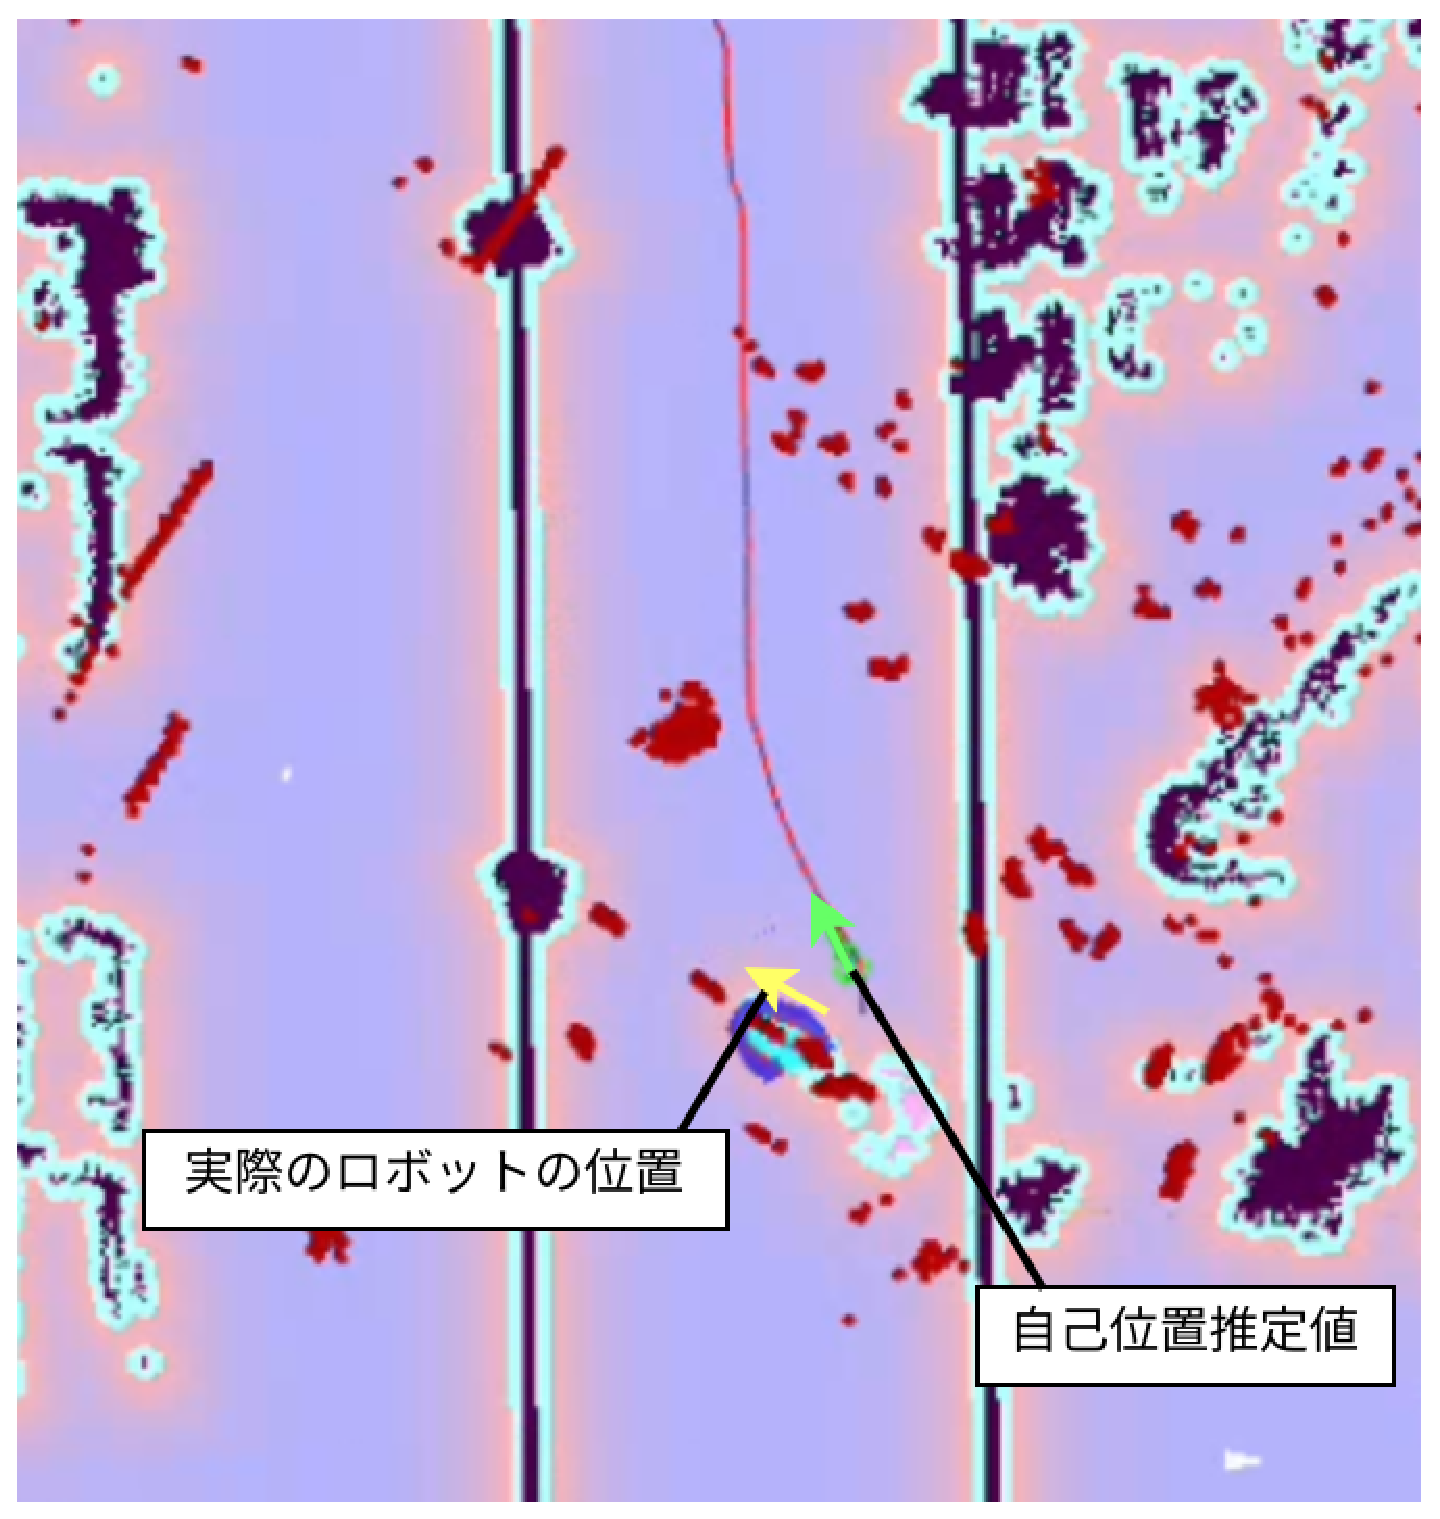
\includegraphics[width=1.0\linewidth]{figs/kinako_result.eps}
    \caption{自己位置推定とナビゲーションが機能しない状況の図}
    \label{fig:kinako_result}
  \end{center}
\end{figure}



\subsubsection{実験走行で発生した問題}
実験走行においては, 以下の技術的な問題が発生した. 

\paragraph{隘路で起きた問題}
実験走行時, 隘路でロボットが回転し止まらなくなることが何度かあった. 
navigation2のログを解析した結果, 以下の処理が行われていたことが確認できた. 

\begin{enumerate}
  \item 障害物との距離が近いためロボットの周囲ローカルコストマップが飽和
  \item ローカルプランナーのパスを生成できずリカバリの動作として回転を開始
  \item  一定時間回転後に速度指令値を0にする処理を実行
\end{enumerate}

しかし, 3の処理が実行されていたにも関わらず, 
実際のロボットは静止せず回転を続けていた. 
このようなバグは除去するかコードにパッチを当てることで可能であるが, 
結局, グローバルプランナーとローカルプランナー, 
リカバリ動作の切り替えが本質的に難しいことも問題となる. 
この問題に関しては文献\cite{ueda2023JRM}で指摘した通りであるので, 
このような切り替えが不要な文献\cite{ueda2023JRM}の方法の
導入を考えなければならない. 
%実際の挙動とシステムの指令値の不一致について, 
%原因を究明するための調査を行っていく予定である. 

\paragraph{動的障害物への対応の遅れ}
動的障害物に対するグローバルパスの更新が遅く, 
オペレーターが緊急停止を押さなければ衝突してしまう場面があった. 
また, システムが動的障害物の進行方向に経路を設定することがあり, 
円滑な走行の妨げとなった. 

このようにプログラム内の各機能が競合するという問題も, 
価値反復や強化学習のように, 
経路ではなく最適方策を求める方法を用いると
(別の問題は発生するかもしれないが, )起こらなくなる. 
逆に言えば経路を求める方法は根本的な問題をはらんでいる. 
小手先ではなく, 根本的な対策が必要となる. 

%これに対する対策として, グローバルプランナーの更新周期の最適化と動的な障害物の移動方向を考慮したグローバルパスの生成のアルゴリズム改良が挙げられる. 
